\chapter{量子估计、Rayleigh 限制和亚分辨信息}
\label{chap:08}

\begin{chapteropening}
Rayleigh 判据给出的是一个成像判据：两个 Airy 斑的主峰是否能在像面上分成两个峰。天文观测中更常见的问题是估计问题：给定一批光子、一个点扩散函数和一个源模型，双星角分离、恒星角直径或亮度矩的误差能小到什么程度。量子估计理论把这个问题写成光场态和测量之间的信息匹配；对弱热光源，直接成像会在亚 Rayleigh 区域丢失一部分分离信息，空间模式测量则可以保留关于分离和尺度的 Fisher 信息 \citep{1925PCPS...22..700F,1969JSP.....1..231H,2000PhRvL..85.3789K,2016PhRvX...6c1033T,2016OExpr..24.3684N,2017NJPh...19b3054T}。
\end{chapteropening}

\section{Rayleigh 判据为什么不是估计极限}

设望远镜口径为 \(D\)，波长为 \(\lambda\)。圆孔衍射的第一个零点在
\begin{equation}
  \theta_{\rm R}=1.22\,\frac{\lambda}{D}
  \label{eq:ch08-rayleigh}
\end{equation}
\begin{formulaexplain}
\(\theta_{\rm R}\) 是 Rayleigh 角尺度；\(\lambda\) 是波长，\(D\) 是口径，系数 1.22 来自圆孔 Airy 斑第一个零点。它给出像面分峰判据，而不是参数估计的最终极限。
\end{formulaexplain}
处。这里 \(\theta_{\rm R}\) 的单位是弧度；乘以 \(206265\times10^3\) 可换成毫角秒。一个 \(D=8~{\rm m}\) 的望远镜在 \(\lambda=500~{\rm nm}\) 时有 \(\theta_{\rm R}\simeq 15.7~{\rm mas}\)，在 \(1.6~\mu{\rm m}\) 时约为 \(50~{\rm mas}\)；一个 \(30~{\rm m}\) 望远镜在 \(500~{\rm nm}\) 时约为 \(4.2~{\rm mas}\)。真实点扩散函数由孔径遮挡、分段镜、像差、自适应光学校正和大气残差共同决定。为了看清解析结构，先采用一维高斯点扩散函数：
\begin{equation}
  h(x)=\frac{1}{\sqrt{2\pi}\sigma}
       \exp\!\left(-\frac{x^2}{2\sigma^2}\right),
  \label{eq:ch08-gaussian-psf}
\end{equation}
\begin{formulaexplain}
\(h(x)\) 是归一化点扩散函数；\(x\) 是像面或角坐标，\(\sigma\) 是宽度。这个高斯模型把真实 PSF 简化成一个可解析的响应核，方便看清分离信息怎样进入数据。
\end{formulaexplain}
其中 \(x\) 是焦平面坐标或等效角坐标，\(\sigma\) 是同一坐标下的点扩散函数宽度。若用角坐标，\(\sigma_\theta\) 的典型量级约为 \(0.4\lambda/D\) 到 \(0.5\lambda/D\)，具体数值要由实测 PSF 或注入源标定给出。

两个等亮、互不相干点源的角分离为 \(s\)，质心放在零点。直接成像记录的是像面光子位置 \(x_i\)，其单光子概率密度为
\begin{equation}
  p(x|s)=\frac{1}{2}h\!\left(x-\frac{s}{2}\right)
        +\frac{1}{2}h\!\left(x+\frac{s}{2}\right).
  \label{eq:ch08-direct-probability}
\end{equation}
\begin{formulaexplain}
\(p(x|s)\) 是给定分离 \(s\) 时单个光子落在 \(x\) 的概率密度；两个 \(h\) 分别来自质心两侧的点源，系数 \(1/2\) 表示等亮。直接成像只看到两个 PSF 的混合。
\end{formulaexplain}
左边的 \(p(x|s)\) 在数据中由归一化图像、事件位置直方图或 PSF 拟合得到，单位是角度的倒数。右边的 \(s\) 和 \(\sigma\) 应使用同一单位。式 \eqref{eq:ch08-direct-probability} 假设两个源等亮、谱形相同、PSF 对两个源相同、背景已扣除或另行建模；若亮度比未知，需要把通量比也放进参数向量。

现在问题变清楚了：Rayleigh 判据问的是像面曲线是否出现两个峰，而估计问题问的是 \(p(x|s)\) 随 \(s\) 改变得有多快。直接图像在 \(s\ll\sigma\) 时几乎不变。把式 \eqref{eq:ch08-direct-probability} 中的两个偏移 PSF 展开，
\[
  h\!\left(x\pm\frac{s}{2}\right)
  =h(x)\pm\frac{s}{2}h'(x)+\frac{s^2}{8}h''(x)+\mathcal{O}(s^3),
\]
放回平均后，一阶项相互抵消，
\[
  p(x|s)=h(x)+\frac{s^2}{8}h''(x)+\mathcal{O}(s^4).
\]
也就是说，双源分离首先表现为 PSF 的二阶展宽，而不是峰位的一阶移动。于是“看不出两个峰”并不等价于“没有任何信息”，但直接像素测量得到的信息确实会迅速下降。对高斯 PSF，分离参数的单光子 Fisher 信息在小分离极限满足
\begin{equation}
  F_{ss}^{\rm direct}\simeq \frac{s^2}{8\sigma^4},
  \qquad s\ll\sigma .
  \label{eq:ch08-direct-small-s}
\end{equation}
\begin{formulaexplain}
\(F_{ss}^{\rm direct}\) 是直接成像对分离 \(s\) 的单光子 Fisher 信息；小分离时它正比于 \(s^2\)。因此两源越接近，像素数据对分离的一阶灵敏度越弱。
\end{formulaexplain}
这里 \(F_{ss}^{\rm direct}\) 的单位是角度的 \(-2\) 次方。若把参数写成无量纲的 \(q=s/\sigma\)，则 \(F_{qq}^{\rm direct}\simeq q^2/8\)。这个二次下降就是 Rayleigh curse：光子数增加当然会降低误差，但在固定光子数下，源越接近，直接成像对分离越不敏感 \citep{2016PhRvX...6c1033T,2018Optic...5.1177P}。

\begin{figure}[tbp]
\centering
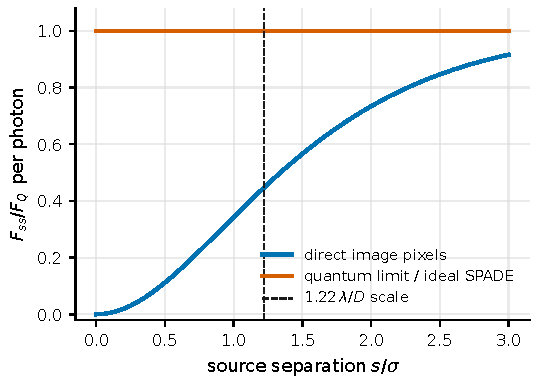
\includegraphics[width=0.82\linewidth]{figures/generated/chapter_08/ch08_rayleigh_information.pdf}
\caption{两个等亮不相干高斯点源的分离信息。蓝线是由像面概率密度 \(p(x|s)\) 数值积分得到的直接成像 Fisher 信息，并按量子 Fisher 信息归一化；橙线表示理想空间模式测量可达到的量子极限。小分离时直接图像的形状变化为二阶小量，因此 \(F_{ss}^{\rm direct}\) 向零下降，而模式测量仍能保留有限信息。虚线标出常用的 Rayleigh 角尺度位置。}
\label{fig:chapter-08-rayleigh-information}
\end{figure}

估计问题和检测问题要分开。若问题是“一个源还是两个源”，模型维数会改变，分离 \(s=0\) 又位在参数空间边界，常规似然比近似未必可靠；若已经接受双源模型，问题才是估计 \(s\)、质心、亮度比和颜色。亚分辨测量依赖给定的参数化模型，用更合适的测量读出已经存在于光场中的信息。对真实天体，模型通常还包括有限角直径、伴星亮度比、谱带差异、偏振、时间变化和背景星污染，这些都会把单参数下界变成多参数协方差问题。

\section{Fisher 信息在比较什么}

一次观测得到 \(N_\gamma\) 个可用于估计的源光子。若背景、坏像素和选择函数已经写进概率密度，直接成像的似然函数可写为
\begin{equation}
  \ln \mathcal{L}(s)=\sum_{i=1}^{N_\gamma}\ln p(x_i|s),
  \label{eq:ch08-direct-likelihood}
\end{equation}
\begin{formulaexplain}
\(\ln\mathcal L(s)\) 是分离 \(s\) 的直接成像对数似然；\(x_i\) 是第 \(i\) 个光子位置，\(N_\gamma\) 是有效源光子数。它把所有光子位置对同一分离模型的支持相加。
\end{formulaexplain}
其中 \(x_i\) 是第 \(i\) 个光子的角位置或像素位置。对应的 Fisher 信息为
\begin{equation}
  F_{ss}=N_\gamma \int
  \frac{1}{p(x|s)}
  \left[\frac{\partial p(x|s)}{\partial s}\right]^2{\rm d}x .
  \label{eq:ch08-fisher-direct}
\end{equation}
\begin{formulaexplain}
\(F_{ss}\) 是总 Fisher 信息；导数 \(\partial p/\partial s\) 衡量分离改变时概率密度变化多快，\(1/p\) 给出统计权重。它把模型灵敏度和光子数合成误差下界。
\end{formulaexplain}
积分变量 \(x\) 的单位和 \(s\) 一致。\(N_\gamma\) 是通过孔径、曝光时间、谱带、总效率和数据选择后留下的源光子数；对于明亮恒星，毫秒到小时曝光可覆盖 \(10^6\) 到 \(10^{12}\) 量级，具体值取决于望远镜面积、滤光片宽度、探测器效率和是否把光分到多个模式或多个基线。若每个像素还有背景 \(b(x)\)，则 \(p\) 要替换成源加背景的归一化混合分布，背景比 \(N_{\rm bg}/N_\gamma\) 从暗场中的 \(\ll 0.01\) 到拥挤星场或强天空背景下的 \(>1\) 都可能出现。

任意无偏估计量 \(\hat{s}\) 的方差满足
\begin{equation}
  {\rm Var}(\hat{s})\ge \frac{1}{F_{ss}} .
  \label{eq:ch08-crb}
\end{equation}
\begin{formulaexplain}
\(\hat s\) 是分离估计量；\({\rm Var}(\hat s)\) 是它的方差。Cramér--Rao 下界说明 Fisher 信息越大，任何无偏估计能达到的最小统计误差越小。
\end{formulaexplain}
若同时估计多个参数 \(\boldsymbol{\theta}=(s,x_0,r,\sigma,b,\ldots)\)，标量下界要换成矩阵形式
\begin{equation}
  {\rm Cov}(\hat{\boldsymbol{\theta}})\succeq F^{-1},\qquad
  F_{\alpha\beta}=N_\gamma\int
  \frac{1}{p(x|\boldsymbol{\theta})}
  \frac{\partial p}{\partial\theta_\alpha}
  \frac{\partial p}{\partial\theta_\beta}\,{\rm d}x .
  \label{eq:ch08-fisher-matrix}
\end{equation}
\begin{formulaexplain}
\({\rm Cov}(\hat{\boldsymbol\theta})\) 是多参数协方差矩阵；\(F_{\alpha\beta}\) 比较参数 \(\theta_\alpha,\theta_\beta\) 对同一数据分布的影响。矩阵逆中的非对角项记录参数退化。
\end{formulaexplain}
\(F^{-1}\) 的非对角项描述退化。比如未知质心会和分离混合，未知亮度比会把一部分偶模式和奇模式信息重新分配，未知 PSF 宽度会把双星分离和普通展宽混在一起。实际报告误差时，通常需要给出统计协方差、PSF 标定误差、背景估计误差和模型误差，而不是只给一个 \(1/\sqrt{F_{ss}}\)。

这时“量子”二字的作用很具体：它不是说望远镜绕过了衍射，而是把测量方式也放进优化问题。经典 Fisher 信息先固定测量，例如像素计数，然后问这些数据对参数有多少灵敏度。量子 Fisher 信息则把“像素测量”替换成“所有量子力学允许的测量”，问同一束光在原则上最多能携带多少可读出的参数信息。

第 \ref{chap:03} 章式 \eqref{eq:ch03-weak-thermal} 已经把弱热光写成真空项加少量一光子项：每个相干时间模式中的平均光子数为 \(\epsilon\ll1\)，大多数时间窗没有点击；没有点击的时间窗不携带角分离信息，真正进入估计的是被探测到的一光子空间模式。两个等亮不相干点源的一光子部分可写成
\begin{equation}
  \rho_1(s)=\frac{1}{2}
  \left|\psi_{+s/2}\right\rangle\left\langle\psi_{+s/2}\right|
  +\frac{1}{2}
  \left|\psi_{-s/2}\right\rangle\left\langle\psi_{-s/2}\right| ,
  \label{eq:ch08-one-photon-state}
\end{equation}
\begin{formulaexplain}
\(\rho_1(s)\) 是探测到一个光子时的空间模式密度矩阵；\(|\psi_{\pm s/2}\rangle\) 是两个源经过望远镜后的场模式。非相干等亮双源表现为两个单光子模式的概率混合。
\end{formulaexplain}
\Needspace{13\baselineskip}
其中 \(\psi_{\pm s/2}\) 是两个源通过望远镜和成像系统后的场振幅模式。对高斯振幅 PSF，在质心、亮度和 PSF 已知的理想情况下，分离的量子 Fisher 信息为
\begin{equation}
  F_{ss}^{Q}=N_\gamma\,\frac{1}{4\sigma^2}.
  \label{eq:ch08-qfi-gaussian}
\end{equation}
\begin{formulaexplain}
\(F_{ss}^{Q}\) 是所有允许测量中可达到的分离信息上限；\(N_\gamma\) 给出光子数增益，\(\sigma\) 给出模式宽度。它在 \(s\to0\) 时不消失，说明信息仍在光场中。
\end{formulaexplain}
它不随 \(s\to0\) 消失。式 \eqref{eq:ch08-qfi-gaussian} 中的 \(\sigma\) 是场模式对应的像面宽度；若用角坐标，它的单位是弧度。这个结果假设光学系统线性、损耗不随分离变化、两个源互不相干且等亮、中心位置已知，并且测量能接近最优空间模式投影 \citep{1969JSP.....1..231H,2016PhRvX...6c1033T,2016OExpr..24.3684N,2017PhRvA..95f3847A}。

\begin{figure}[tbp]
\centering
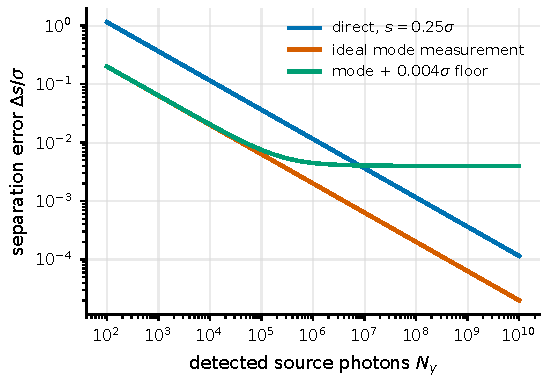
\includegraphics[width=0.82\linewidth]{figures/generated/chapter_08/ch08_cramer_rao_bound.pdf}
\caption{亚分辨双点源的 Cramér--Rao 分离误差。横轴为探测到的源光子数 \(N_\gamma\)，纵轴为 \(\Delta s/\sigma\)。在 \(s=0.25\sigma\) 的例子中，直接成像因 Fisher 信息已经很小，需要更多光子才能达到同样误差；理想模式测量按 \(N_\gamma^{-1/2}\) 下降。绿色曲线加入 \(0.004\sigma\) 的模式匹配系统误差后出现平台，表示继续增加光子数也不能消除标定误差。}
\label{fig:chapter-08-crb}
\end{figure}

量子下界不是自动可达的观测精度。若质心误差为 \(\delta x\)，第一阶模式会得到约 \(\delta x^2/(4\sigma^2)\) 的漏光；而双源分离信号本身在小分离时约为 \(s^2/(16\sigma^2)\)。因此当 \(\delta x\sim s/2\) 时，指向和质心标定已经和待测信号同量级。若 Strehl 比低、像差随时间变化、模式排序器串扰矩阵不稳定，或背景光没有同样的空间模式分布，式 \eqref{eq:ch08-qfi-gaussian} 给出的下界会被系统误差平台取代。实验相位板、PSF shaping 和 SPLICE 类测量表明，非理想但较简单的相位敏感测量也能缓和直接成像的二次信息损失，不过通常仍要靠可见度、串扰和对准误差来决定实际增益 \citep{2017PhRvL.118g0801T,2019NJPh...21i3010B,2018Optic...5.1177P}。

\section{空间模式测量怎样把小分离变成计数}

直接成像把每个光子投影到位置本征态，因此小分离只留下非常弱的形状展宽。空间模式测量换了一个问题：不先问光子落在哪个像素，而是先问它属于哪个正交空间模式。SPADE 把光场先分解到一组空间模式，再对每个模式计数。对于高斯 PSF，最自然的基底是 Hermite--Gaussian 模式。若质心已知且两个点源等亮，理想模式排序给出
\begin{equation}
  p_n=\exp(-Q)\frac{Q^n}{n!},\qquad
  Q=\frac{s^2}{16\sigma^2},
  \label{eq:ch08-spade-probability}
\end{equation}
\begin{formulaexplain}
\(p_n\) 是第 \(n\) 个 Hermite--Gaussian 模式的点击概率；\(Q\) 是由分离 \(s\) 和宽度 \(\sigma\) 构成的无量纲信号强度。SPADE 把分离转成低阶模式的计数分布。
\end{formulaexplain}
其中 \(p_n\) 是第 \(n\) 个 Hermite--Gaussian 模式的单光子概率。\(p_0\) 接近 1，表示绝大多数光仍在基模；\(p_1\simeq s^2/(16\sigma^2)\)，表示一个很小但可计数的奇模式漏出。这个漏出来自两个相互重叠的源模式在空间模式基底中的几何结构，是分离信号的一部分。对 \(N_\gamma\) 个光子，第一阶模式的期望计数为
\begin{equation}
  \langle n_1\rangle\simeq N_\gamma\,\frac{s^2}{16\sigma^2}.
  \label{eq:ch08-first-mode-count}
\end{equation}
\begin{formulaexplain}
\(\langle n_1\rangle\) 是第一阶模式的期望光子数；它等于总源光子数乘以小分离漏入该模式的概率。即使概率很小，大 \(N_\gamma\) 也能把它变成可测计数。
\end{formulaexplain}
例如 \(s=0.1\sigma\) 时，\(p_1\simeq6.25\times10^{-4}\)；若有效源光子数为 \(10^8\)，理想情况下第一阶模式中有约 \(6.3\times10^4\) 个光子。若通量只有 \(10^5\) 个光子，则期望计数约 63 个，暗计数、串扰和背景就会变成主要限制。

\begin{figure}[tbp]
\centering
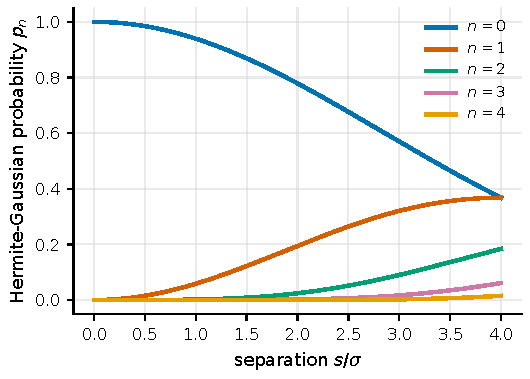
\includegraphics[width=0.82\linewidth]{figures/generated/chapter_08/ch08_spade_probabilities.pdf}
\caption{理想 Hermite--Gaussian 模式排序的模式概率。横轴是源分离 \(s/\sigma\)，纵轴是每个模式的单光子概率。小分离时 \(p_0\) 仍接近 1，但 \(p_1\) 和更高模式按 \(Q=s^2/(16\sigma^2)\) 的幂次增长；分离信息由这些低概率模式的计数携带。}
\label{fig:chapter-08-spade-probabilities}
\end{figure}

图像中的“看不出”可以同时出现在像面曲线和模式概率中：像面轮廓几乎重合，但低概率模式已经变成可测计数。若模式计数服从 Poisson 或 multinomial 统计，模式测量的 Fisher 信息为
\begin{equation}
  F_{ss}^{\rm mode}
  =N_\gamma\sum_n \frac{1}{p_n}
  \left(\frac{\partial p_n}{\partial s}\right)^2 .
  \label{eq:ch08-mode-fisher}
\end{equation}
\begin{formulaexplain}
\(F_{ss}^{\rm mode}\) 是模式计数给出的分离 Fisher 信息；求和覆盖所有空间模式。每一项用模式概率对 \(s\) 的变化率除以该模式的计数噪声，累加成总信息。
\end{formulaexplain}
在小分离极限，仅 \(n=1\) 模式就给出接近 \(N_\gamma/(4\sigma^2)\) 的信息。\(p_1\) 本身随 \(s^2\) 变小，但 \(\partial p_1/\partial s\) 也随 \(s\) 变小，两者在 Fisher 信息中相除后留下有限极限。模式测量由此避开 Rayleigh curse \citep{2016PhRvX...6c1033T,2017NJPh...19b3054T}。

\begin{figure}[tbp]
\centering
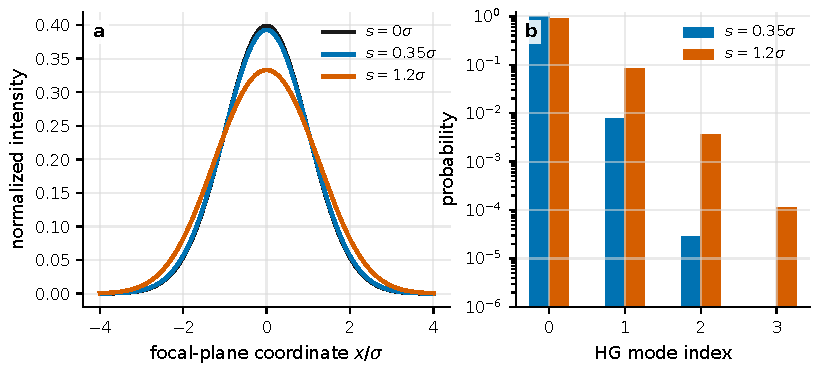
\includegraphics[width=0.92\linewidth]{figures/generated/chapter_08/ch08_direct_image_vs_modes.pdf}
\caption{同一双源模型在直接像面和模式输出中的表现。左图显示 \(s=0\)、\(0.35\sigma\) 和 \(1.2\sigma\) 的归一化像面强度；亚分辨分离时曲线差别主要表现为很弱的展宽。右图显示 \(s=0.35\sigma\) 和 \(1.2\sigma\) 的前四个 Hermite--Gaussian 模式概率；低阶非基模概率虽小，却把分离信息变成了模式计数。}
\label{fig:chapter-08-direct-vs-modes}
\end{figure}

天文实现还要处理二维分离、偏振、谱带和光学耦合。二维问题把 \(s\) 换成 \((s_x,s_y)\)，相应模式变成二维 Hermite--Gaussian 或与真实孔径匹配的正交模式；角分离的两个方向在圆对称 PSF 下有相同量级的 QFI，但非圆 PSF、分段镜和像差会引入方向依赖 \citep{2017PhRvA..95f3847A}。广义 SPADE 可估计亚衍射目标的二阶及更高空间矩，但高阶矩需要更高阶模式，光子数需求迅速上升，有限矩也不能唯一重建任意亮度分布 \citep{2017NJPh...19b3054T}。因此星对、近距离伴星、恒星形状和少参数亮度矩是更自然的应用；复杂盘面、喷流和星云需要把模式测量和常规成像、振幅干涉或强度干涉联合起来。

部分相干性会改变模式概率。Larson 和 Saleh 讨论了部分相干源中 Rayleigh curse 重新出现的条件；Tsang 和 Nair 随后指出，对弱热光和正确的 SPADE Fisher 计算，只要不是完全正相关的退化情形，模式测量仍可避免小分离信息完全消失 \citep{2018Optic...5.1382L,2019Optic...6..400T}。在天文学里要特别区分两件事：源面上两个辐射区域是否独立发光，以及传播到望远镜后由 van Cittert--Zernike 定理产生的空间相干。后者正是一阶或二阶干涉测量的目标，不应简单等同于源本身的相干发射。

\section{强度干涉怎样把角尺度写进长基线数据}

前一节讨论的是单孔径或相干合束后的空间模式测量。长基线阵列把同一个估计问题放到 Fourier 平面：不同望远镜对采样不同空间频率，数据约束来自可见度随基线的变化。这里的“亚分辨”不是从单个 Airy 斑里读出两个峰，而是在长基线上测量源亮度分布的 Fourier 模长。

强度干涉不测一阶场相位，而测不同望远镜光强涨落的相关。理想热光下，零延迟二阶相关给出
\begin{equation}
  g_{ij}^{(2)}(0)-1 = |\gamma_{ij}|^2,
  \label{eq:ch08-hbt-g2}
\end{equation}
\begin{formulaexplain}
\(g_{ij}^{(2)}(0)\) 是两台望远镜零延迟二阶相关；\(\gamma_{ij}\) 是归一化复相干度。热光 HBT 关系说明强度涨落相关直接给出可见度模平方。
\end{formulaexplain}
其中 \(\gamma_{ij}\) 是望远镜 \(i,j\) 之间的复相干度，等于归一化一阶可见度 \(V(u,v)\)。在有限时间 bin、有限光谱带宽和探测器响应下，实测对比度会被相干时间与电子时间分辨率的比值稀释；分析通常直接拟合校准后的 \(|V|^2\) 和它的协方差。HBT 实验和 Narrabri 强度干涉仪正是用这种方式测量恒星角直径，现代 Cherenkov 望远镜阵列则把大收集面积和数字相关器带入同一问题 \citep{1956Natur.177...27B,1956Natur.178.1046H,1957RSPSA.242..300B,1974iiia.book.....H,1974MNRAS.167..121H,1974MNRAS.167..475H,2008AIPC..984..205L,2013APh....43..331D,2015NatCo...6.6852D,2020NatAs...4.1164A,2024MNRAS.529.4387A}。

若观测量是若干基线和谱道上的
\begin{equation}
  d_k=|V(u_k,v_k;\boldsymbol{\theta})|^2+\eta_k ,
  \label{eq:ch08-sii-data}
\end{equation}
\begin{formulaexplain}
\(d_k\) 是第 \(k\) 个基线/时间/谱道上的平方可见度数据；\(V\) 是模型可见度，\(\boldsymbol\theta\) 是源参数，\(\eta_k\) 是噪声。强度干涉把角结构写进 \(|V|^2\) 的基线变化中。
\end{formulaexplain}
其中 \(k\) 标记基线、时间、谱道或偏振通道，\(\eta_k\) 是噪声项，则参数 \(\theta_\alpha\) 的 Fisher 矩阵可写成
\begin{equation}
  F_{\alpha\beta}^{\rm SII}
  =\sum_{k,l}
  \frac{\partial |V_k|^2}{\partial\theta_\alpha}
  C^{-1}_{kl}
  \frac{\partial |V_l|^2}{\partial\theta_\beta}.
  \label{eq:ch08-sii-fisher}
\end{equation}
\begin{formulaexplain}
\(F_{\alpha\beta}^{\rm SII}\) 是强度干涉数据的 Fisher 矩阵；\(C^{-1}_{kl}\) 按数据协方差给权重。可见度模平方对参数变化越陡、误差越小，对应参数信息越多。
\end{formulaexplain}
\(C_{kl}\) 是 \(|V|^2\) 测量误差协方差，可由时间移位背景、空基线、夜间重复观测或注入模拟估计。若误差近似独立，式 \eqref{eq:ch08-sii-fisher} 退化为每个数据点的斜率平方除以方差。对均匀圆盘恒星，
\begin{equation}
  V(x)=\frac{2J_1(x)}{x},\qquad
  x=\pi B\theta_\star/\lambda ,
  \label{eq:ch08-uniform-disk-visibility}
\end{equation}
\begin{formulaexplain}
\(V(x)\) 是均匀圆盘的可见度；\(J_1\) 是一阶 Bessel 函数，\(B\) 是投影基线，\(\theta_\star\) 是角直径。基线通过 \(x\) 扫描圆盘亮度分布的 Fourier 模长。
\end{formulaexplain}
\(B\) 是投影基线，\(\theta_\star\) 是角直径。对 \(\theta_\star\) 最有用的基线通常落在 \(|V|^2\) 斜率大的区域；短基线平台上模型变化太小，极长基线上信号又容易被系统误差压住。

\begin{figure}[tbp]
\centering
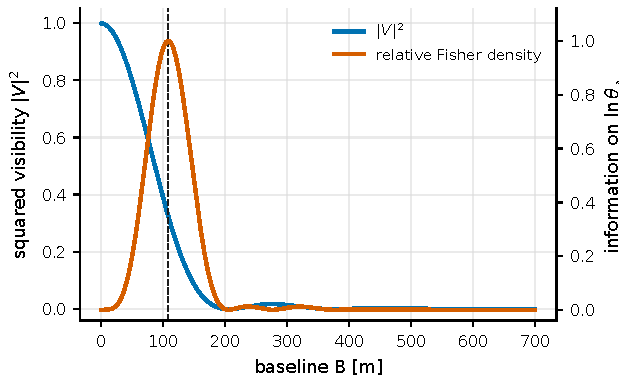
\includegraphics[width=0.82\linewidth]{figures/generated/chapter_08/ch08_visibility_fisher_design.pdf}
\caption{强度干涉中基线选择和参数信息的关系。蓝线为 \(\lambda=450~{\rm nm}\)、\(\theta_\star=0.55~{\rm mas}\) 均匀圆盘模型的平方可见度；橙线为按 \(\partial |V|^2/\partial\ln\theta_\star\) 计算并归一化的 Fisher 权重。最有用的基线位在可见度快速下降处，单纯增加或缩短基线都不会自动增加角直径信息。}
\label{fig:chapter-08-sii-fisher}
\end{figure}

强度干涉的代价是相位缺失。\(|V|^2\) 对整体平移不敏感，也会产生镜像和中心对称退化；二元星的方向、亮斑位置和非对称盘面结构往往需要地球自转覆盖、多波长信息、先验模型或三阶相关来缓解。它的优势是对大气相位扰动不敏感，望远镜之间只需电子连接，不必保持光学相干。现代时间标记器和高速相关器可以处理许多通道，但可用 Fisher 信息仍受光子率、电子带宽、背景、时间同步、基线覆盖和系统协方差限制 \citep{2017MNRAS.472.4126G,2020RScI...91a3108W,2020NatAs...4.1164A,2024MNRAS.529.4387A}。

\section{天文应用中怎样避免误读量子极限}

模式测量和强度干涉面对的是不同的工程瓶颈。SPADE、SLIVER 和相位敏感测量通常要求单孔径或相干组合后的稳定波前，适合把目标光耦合进光纤模式、集成光学芯片或自由空间模式排序器。自适应光学把入射光尽量压到可控的少数空间模式中；Strehl 比、非共路像差、色散和偏振串扰都会进入模式响应矩阵。强度干涉接受大气相位随机化，用大收集面积和长基线换取 \(|V|^2\) 信息，更适合亮热星、快速旋转星、双星和角直径测量。

一套可用于科学结果的亚分辨估计需要同时交代光子预算、角尺度、测量矩阵、模型边界和误差拆分。光子预算包括目标星等、谱带、总效率、曝光时间和有效 \(N_\gamma\)；角尺度包括 \(\lambda/D\)、PSF 宽度 \(\sigma_\theta\)、候选分离 \(s\) 或角直径 \(\theta_\star\)。测量矩阵可以是像素响应、模式串扰、\(|V|^2\) 协方差或时间相关背景。模型边界要说明等亮双源、未知亮度比、有限圆盘、部分相干、背景星和时间变化怎样改变 Fisher 矩阵。误差拆分则检查统计项是否按 \(N_\gamma^{-1/2}\) 下降；若误差不再下降，通常是对准、PSF、背景、相关器或模型误差进入平台。

贝叶斯采样和证据比较常用于把这些边界放入最终推断。直接成像、模式计数和强度干涉数据可以共享同一个参数向量，并用联合似然相乘；若要比较单源和双源模型，需要用模拟校准、后验预测检验或证据，而不是简单套用高斯近似。对亚分辨问题，先验会直接改变可识别参数空间：已知轨道、颜色、光谱型、距离、伴星亮度比或恒星演化模型都能改变最终约束 \citep{2009MNRAS.398.1601F,2013PASP..125..306F}。

